\chapter{Placas, configuración para las lecturas y primeras muestras}
\label{chap:cap1}

\lettrine Cual sería entonces la forma de leer estas señales de forma fácil? Esta fue la pregunta que me hice y mi primer recurso de información para responderla fue internet. Indagando encontré que existían algunos fabricantes estadounidenses de PCBs para desarrollo que ofrecían soluciones de difícil acceso y a coste alto. Por ello seguí buscando y topé con un canal llamado "Biomakers" en donde había tutoriales muy buenos sobre EMG, ECG, EEG, e incluso, enseñaba diseños para la circuitería necesaria. Quiero comenzar este capítulo entonces hablando a grandes rasgos de la composición de los mismos ya que me sorprendió lo sencillos que son. El principio básico de un sensor se trata en mapear una magnitud real como la luz, la temperatura u otros en funciones matemáticas, extraemos valores del mundo que nos rodea para poder representarlos de forma transductible. En este caso al estar leyendo los pocos milivoltios que se generan durante la actividad muscular, entre nuestra señal y sensor no existirá la necesidad de hacer transformaciones entre magnitudes ya que simplemente servirá como amplificador de la actividad para obtener un señal manipulable.

\begin{figure}[hp!]
\begin{center}
    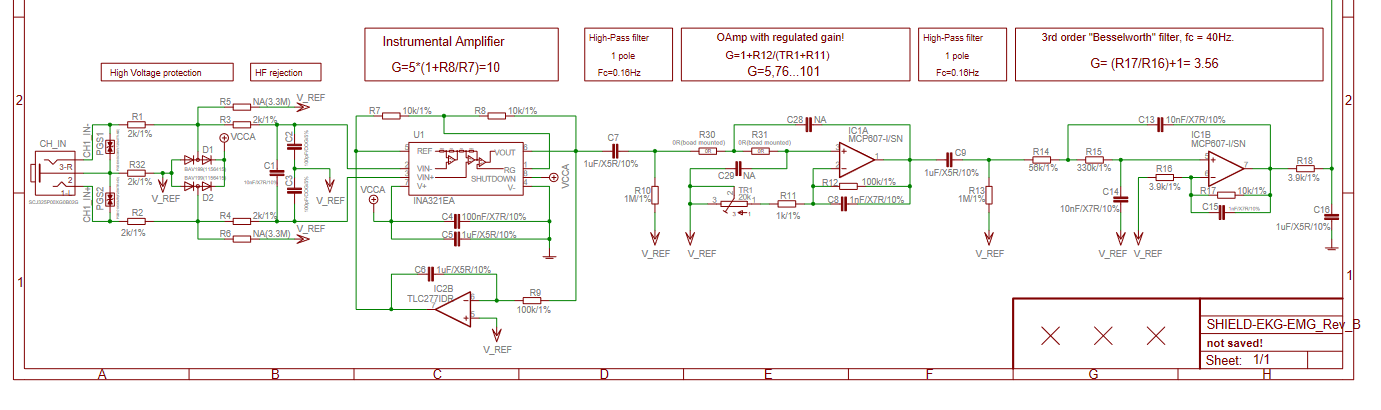
\includegraphics[width=0.95\textwidth,scale=0.5, height=5.5cm]{imaxes/circuito.png}

  \end{center}
\end{figure}

El circuito de la figura hace referencia a la placa SHIELD-EKG-EMG de Olimex, como su nombre indica se trata de un "escudo" que se puede apilar sobre las placas de tipo Arduino Uno y cuenta con todos los componentes para ser calibrada y conectada a la misma. Esta parte de su esquemático se corresponde con la del sensor electromiográfico. 

Empezando desde las izquierda del todo vemos que existe una conexión "CH\_IN" en donde tenemos 3 terminales de conexión L, R y Masa, correspondiéndose cada uno con los terminales de los 3 electrodos. A grandes rasgos, lo que podemos ver es que las corrientes recogidas por estos elementos irán pasando por varias fases de amplificación y filtrado. Comenzando por componentes de protección pasamos a una etapa en donde rechazaremos frecuencias altas y a continuación, amplificaremos la señal mediante un Amplificador Operacional de cierta ganancia. Seguimos entonces con etapas de filtrado para la frecuencia de 0 Hz característica de la corriente continua para finalmente, llegar a una etapa que creo merece cierta explicación.

En este caso se trata de una fase en donde utilizaremos un Amplificador de ganancia regulada. Y porque regulada? Bien, durante la introducción explicaba que este tipo de sensores va a estar afectado por ciertas características físicas de la persona y puede ocurrir, que no tenga la sensibilidad suficiente para recoger señales desde la superficie (ya sea por el índice de grasa que separa el sensor y el músculo o también por la poca masa muscular de la zona). Por esto mismo la PCB de Olimex nos permite adaptarnos a cualquier situación. La calibración para esta placa en mi opinión es un poco engorrosa ya que se hace de forma física y mediante una señal PWM que genera, por lo que sería interesante que se pudiese hacer de manera completamente Software.

Pasando a la configuración de sensores y microcontroladores que se utilizó para este proyecto, el sensor de Olimex no fue el único componente que utilicé para los experimentos y en realidad, los resultados que figurarán aquí se corresponden con otra placa. Esto también merece explicación ya que antes de descubrir la antes descrita, un día tuve la suerte de toparme con la siguiente PCB de China.

\begin{figure}[hp!]
\begin{center}
    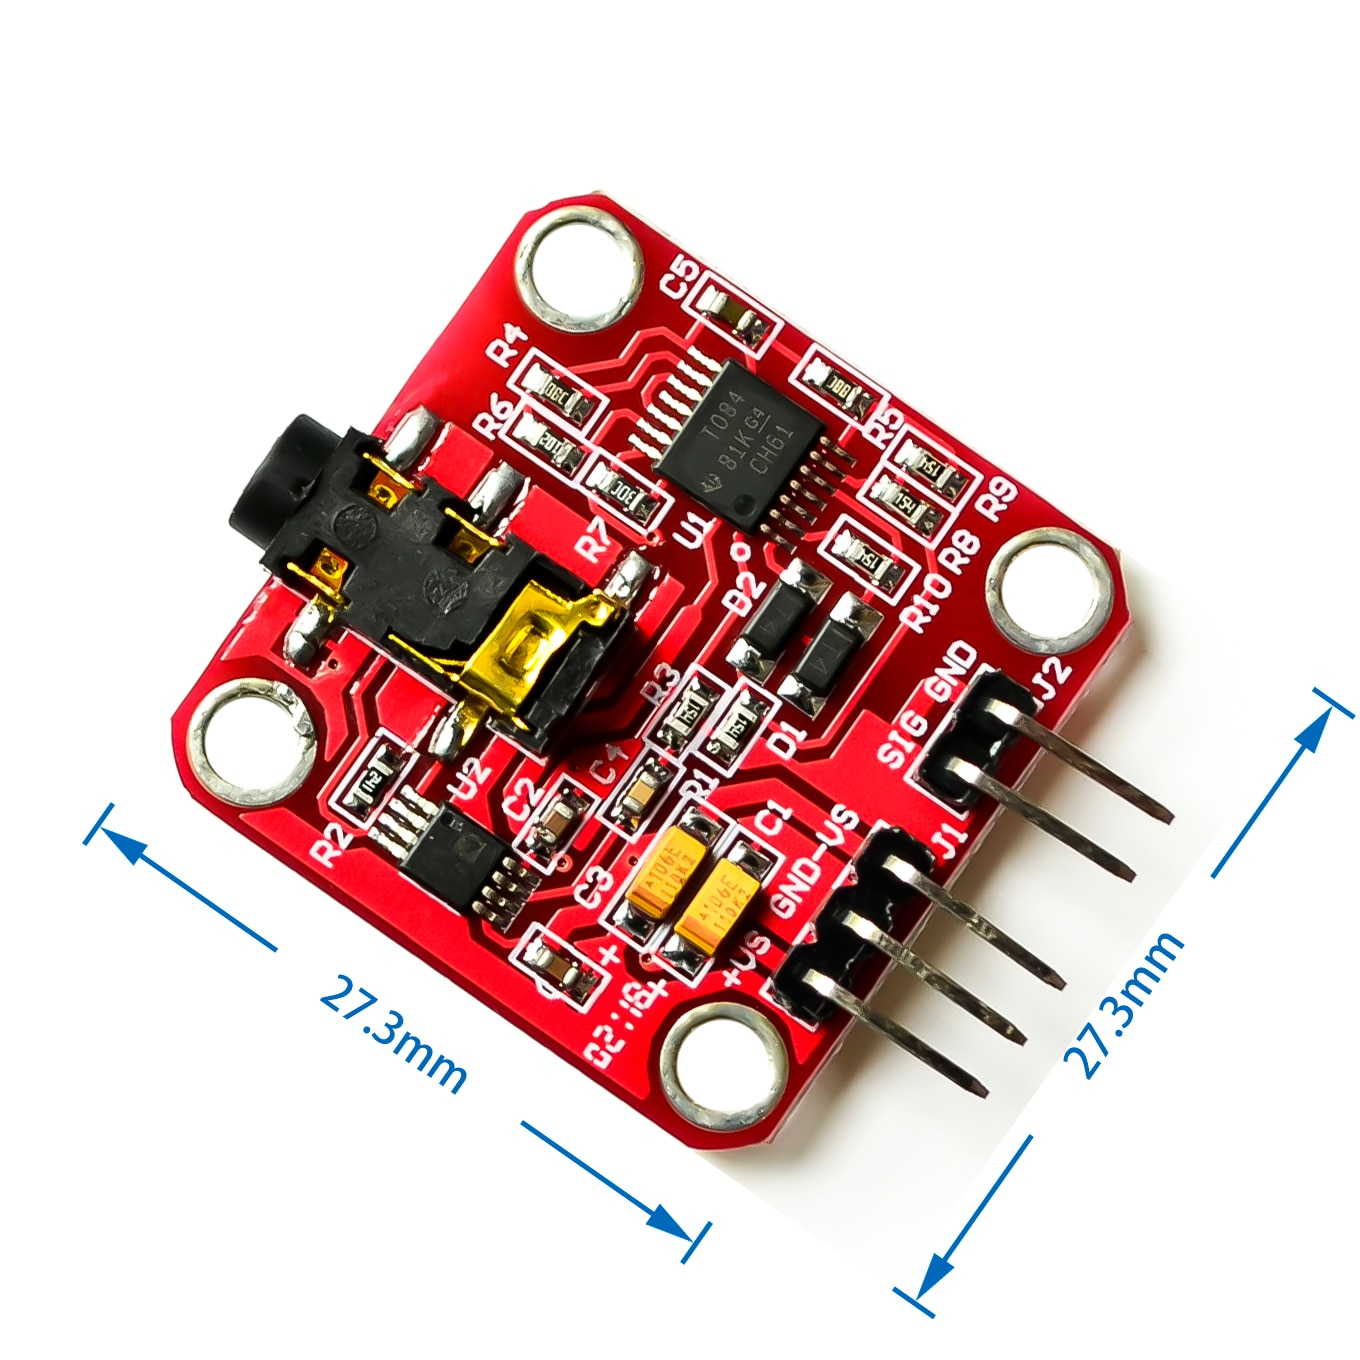
\includegraphics[width=0.6\textwidth, height=5cm]{imaxes/placa_china.jpg}
    \caption{ActionButton}
    \label{fig:plot}
  \end{center}
\end{figure}

Concretamente la encontré en Aliexpress y por 15€, trae un pack con los electrodos, parches y sensor. Desde que me llegó y la probé me di cuenta de que era la indicada para este proyecto, el precio es irresistible, el tamaño y la utilidad que ofrece es muy buena, además, es muy fácil de poner a funcionar. Para ello necesita una alimentación de +9v y -9v, utiliza la referencia positiva y negativa para hacer operaciones, la salida la da por el terminal de "sig" y se trata de una señal analógica de entre 0v y 3v, es decir, completamente positiva (esto tiene sentido porque el Arduino es incapaz de leer voltajes negativos en sus terminales analógicos).    
\vspace{0.15cm}

Por lo tanto contamos con el siguiente Setup para los experimentos:
\begin{itemize}
  \item 2 Placas PCB.
  \item Arduino UNO.
  \item Electrodos en seco y húmedos.
\end{itemize}

\begin{figure}[hp!]
\begin{center}
    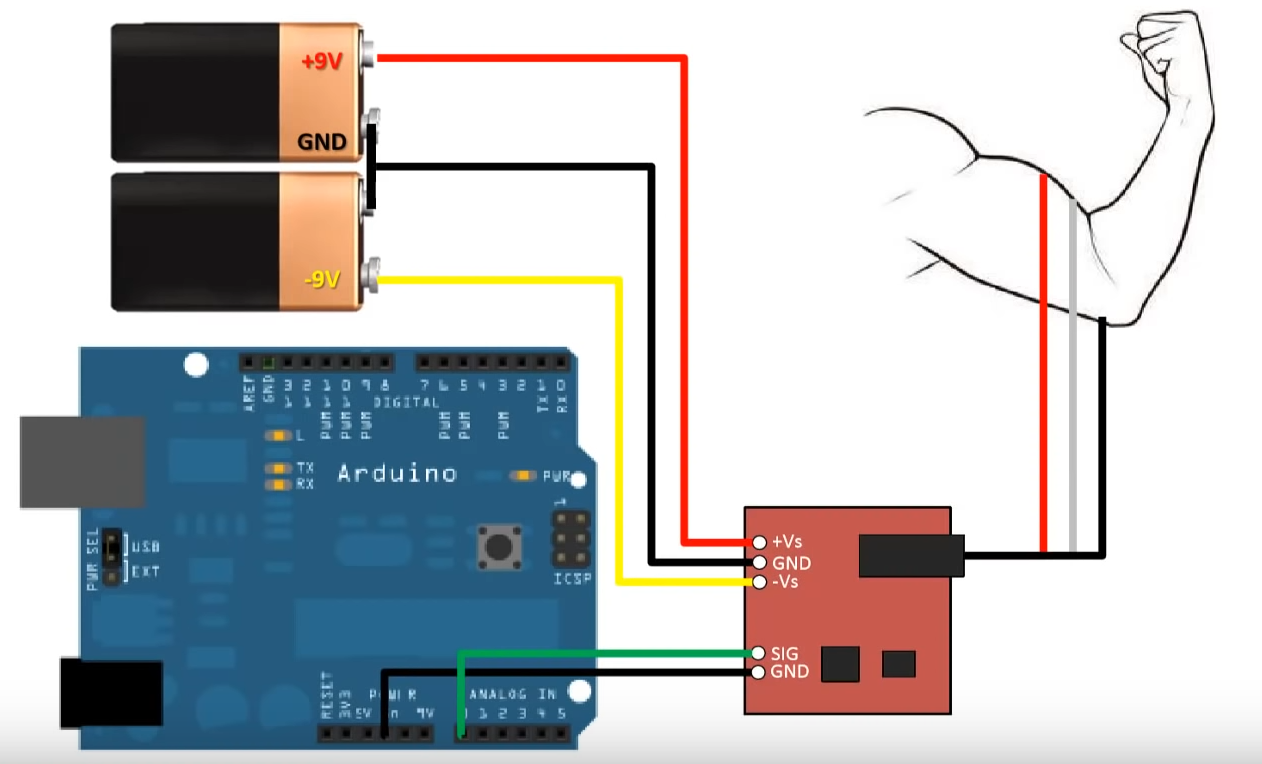
\includegraphics[width=100mm, height=5cm, scale=0.5]{imaxes/montaje.png}
    
    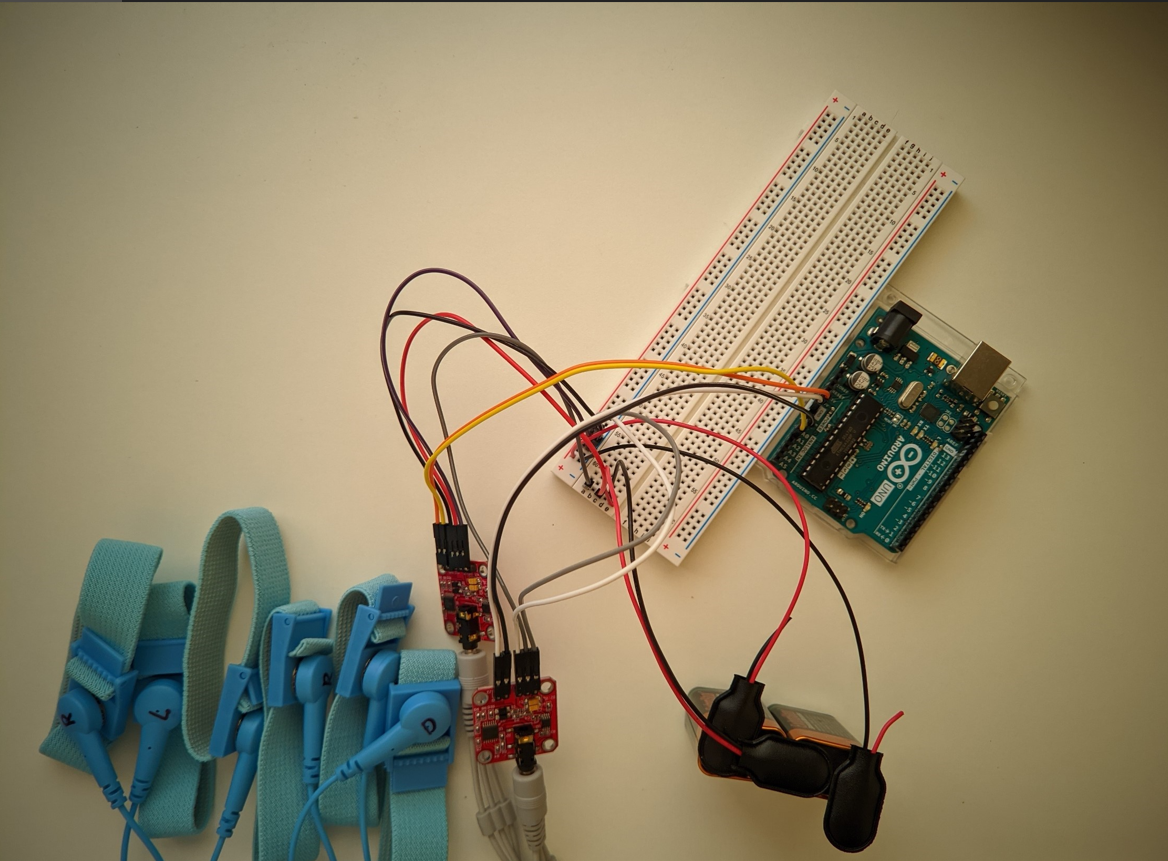
\includegraphics[width=12.5cm, height=6.5cm, scale=0.5]{imaxes/configuracion.png}
    \caption{ActionButton}
    \label{ActionButton}
  \end{center}
\end{figure}

El montaje es bastante trivial, lo puede hacer cualquiera en casa y con un kit de principiantes para electrónica. Se puede ver que que con 10 cables estaría todo montado, por lo que sería muy fácil con este tamaño e incluso un Arduino del tipo Nano diseñar una carcasa a impresora 3d, para acoplarlo todo de forma cómoda.

Después de habernos colocado los electrodos, comenzar a leer los primeros valores es tan fácil como configurar en el código del Arduino el puerto serial y leer dentro del loop por los puertos Analógicos. Aclarando ahora que no voy a entrar en detalles sobre el código ya que es muy simple el funcionamiento y todo estará completamente disponible in mi GitHub.\\ 

\begin{figure}[hp!]
\begin{center}
    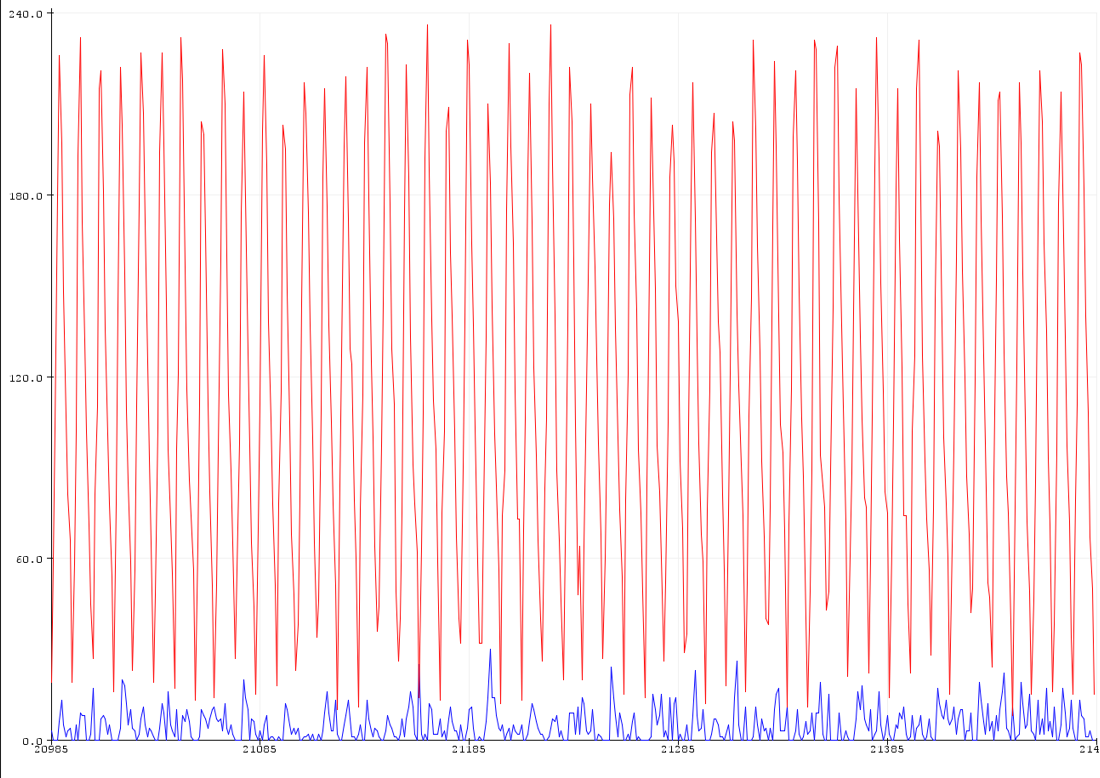
\includegraphics[width=0.75\textwidth, scale=0.5]{imaxes/resting.png}
    \caption{ActionButton}
    \label{fig:plot}
  \end{center}
\end{figure}

La figura \autoref{fig:plot} se trata de un ejemplo de dibujo para las 2 señales de nuestros músculos en reposo, se trata de un plot en tiempo real que nos muestra la herramienta de Serial Plotter y que trae el IDE de Arduino.

Para todos los experimentos configuramos una frecuencia de muestreo a 1000 Hz y BaudRate de 115200. El porqué del primer parámetro se basa en las siguientes 2 ideas:

\begin{itemize}
  \item Las frecuencias significativas en el EMG se encuentran entre los 0Hz y los 500Hz, siendo esta última una opción también para configurar y evitar Aliasing. 
  \item Si se quieren buenos resultados en la prótesis, la respuesta como aplicación de ingeniería debe ser menor a los 300ms, por lo que haciendo cálculos unas 250 muestras serían suficientes para extraer patrones. 
\end{itemize}

Añadir que aunque buscamos buenos resultados con 250 muestras, es recomendable en las mediciones capturar muchas más para tener de sobra durante los análisis.\\ 
Para las mediciones finales, se creó una herramienta Software en Python que se encarga de conectarse al Arduino, sincronizarse con él, leer las muestras de los 2 canales y exportarlas a CSV. A parte de estos comportamientos, también ofrece un menú simple por comandos en el que se puede gestionar el tipo de medición que estamos haciendo, llevar la cuenta de las mismas, plottear el resultado e incluso interaccionar con el usuario mediante un sonido para indicarle cuando debe realizar el movimiento.

Una vez tenemos todo configurado podemos pasar a relizar las primeras mediciones, empezaremos entonces con los siguientes 3 estados:

\begin{itemize}
  \item Flexión de muñeca. 
  \item Extensión de muñeca.
  \item Reposo.
\end{itemize}

\begin{figure}[!h]
  \centering
  \begin{tabular}[c]{cc}
    \begin{subfigure}[c]{0.5\textwidth, scale=0.5}
      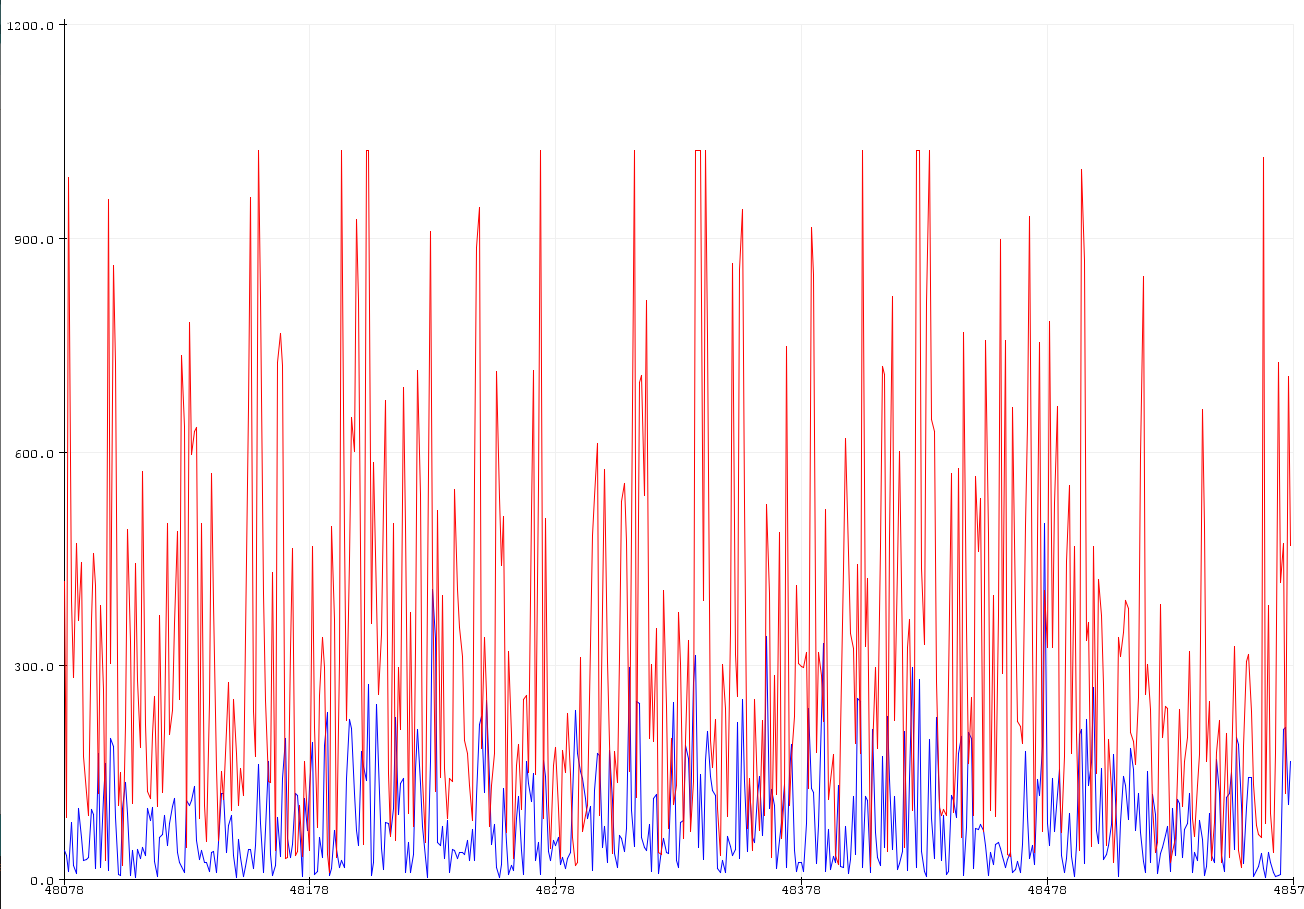
\includegraphics[width=\textwidth]{imaxes/flexion.png}
      
    \end{subfigure}&
    \begin{subfigure}[c]{0.5\textwidth, scale=0.5}
      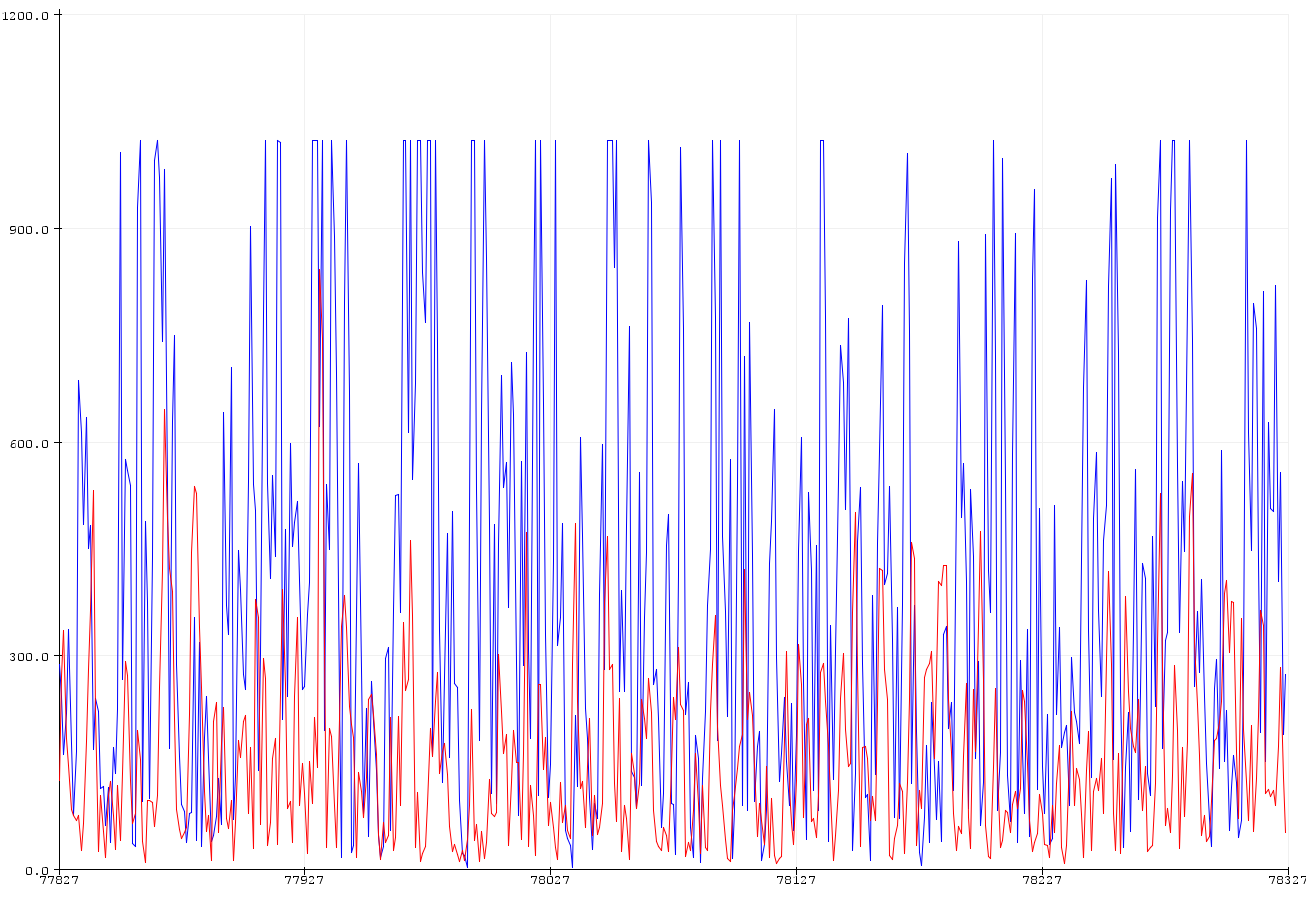
\includegraphics[width=\textwidth]{imaxes/extension.png}
      
    \end{subfigure}&
    \begin{subfigure}[c]{0.5\textwidth, scale=0.5}
      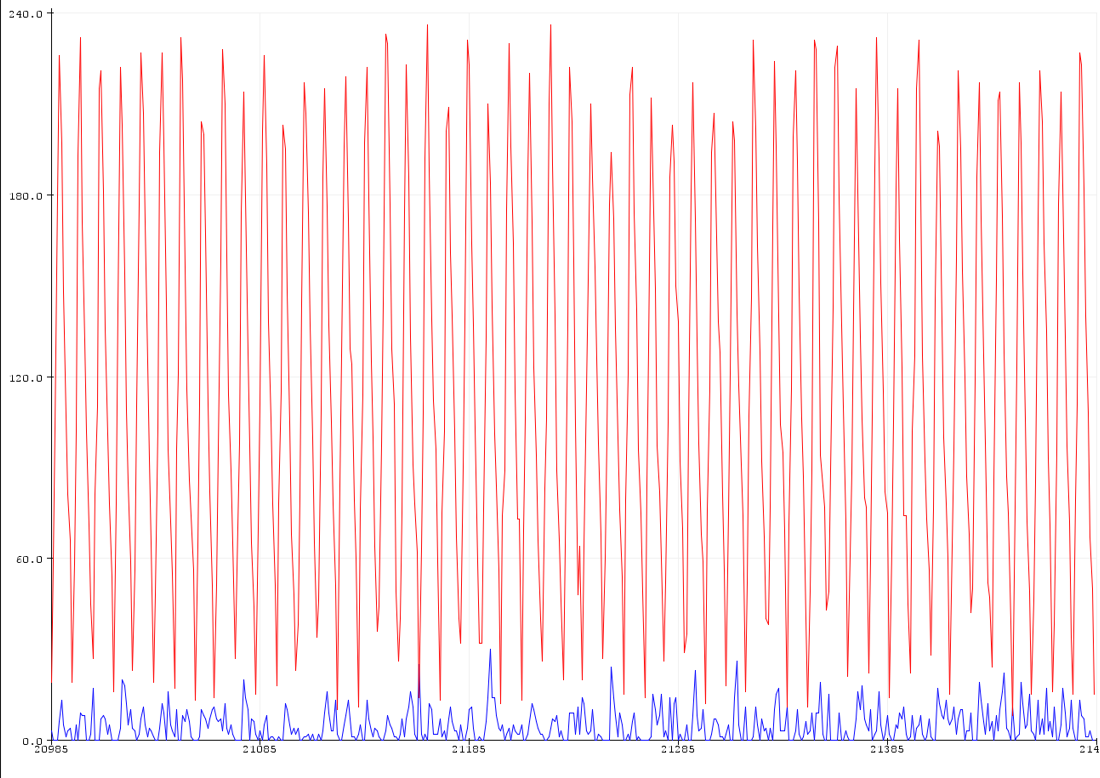
\includegraphics[width=\textwidth]{imaxes/resting.png}
      
    \end{subfigure}\\
    \caption{ActionButton}
  \end{tabular}    
 
\end{figure}

Como se puede ver a simple vista podemos apreciar una diferencia notable entre los 3 movimientos. La línea de plot azul se corresponde con el canal 1 y el músculo 



